\section{Extensions}
\label{sec:extensions}

In section \ref{sec:approach} 
  we made some simplifications in order to keep the discussion brief.
We discuss three extensions to our base approach.
The first extension provides further details on how to assess
  identity conditions of typed literals, which may occur in the object
  position of a triple.
The second extension generalizes the notion of a
  predicate, allowing more indiscernibility predicates to be found.
The third extension shows that definitions
  \ref{def:identity_lower_approximation} and
  \ref{def:identity_higher_approximation}
  do not give the most optimal solution in some arcane cases.

\subsection{Identity of typed literals}

In order to deal with predefined datatypes such as integers, dates, etc.,
  RDF introduces the notion of ``typed literals''.
For such typed literals, identity does not suffice in order to ascertain
  that the sets of object terms denote the same resources
  (definition \ref{def:indiscernibility_properties}).
The reason for this is that typed literals have special identity conditions.
Since typed literals are quite common in SW data, we elaborate on this here.
Roughly speaking, for typed literals we assume a lexical-to-value mapping
  \cite{Hayes2004}, which assigns a value to each lexical expression.
For each datatype we assume a datatype-specific identity relation
  partitioning the datatype's value space.
Identity between typed literals is then defined
  as the datatype-specific identity between the values of the literals
  under the lexical-to-value mapping.
This extension was already used to perform the computational
  experiment of section \ref{sec:experiment}.

\begin{comment}
First we assume a datatype map
  \mbox{$D : \mathcal{I} \rightarrow ICEXT(I({\small \texttt{rdfs:Datatype}}))$},
  where $ICEXT$ is the functional map from classes onto their instances.
Second, for each datatype $d$ we assume a lexical-to-value mapping
  $L2V(d)$,\cite{Hayes2004},
  %: V(d) \rightarrow LEX(d)
  which assigns a value to each lexical expression.
Finally, for each datatype $d$ we assume a datatype-specific identity relation
  $\sim_d$ partitioning the datatype's value space $V(d)$.\footnote{
    Relation $\sim_d$ poses some problems to implement correctly,
      see section \ref{sec:implementation} for details.
    }

Suppose that two objects $o_1$ and $o_2$ are both typed literals,
  with $o_1 = \pair{d_1}{x_1}$ and $o_2 = \pair{d_2}{x_2}$
  for datatype names $d_1$ and $d_2$ and value names $x_1$ and $x_2$.
Identity between $o_1$ and $o_2$ is then defined as in
  \ref{def:identity_typed_literals}.

\begin{definition}[Identity for typed literals]
\label{def:identity_typed_literals}
\begin{align}
  o_1 \approx o_1
\,\iff\,
    D(d_1) = D(d_2)
  & \; \land \; &\nonumber\\
    x_1 \in LEX(d_1)
  & \; \land \; &\nonumber\\
    x_2 \in LEX(d_2)
  & \; \land \; &\nonumber\\
    l2v(D(d_1))(x_1) \sim_d l2v(D(d_2))(x_2)\nonumber
\end{align}
\end{definition}

\noindent Notice that the datatype-specific lexical-to-value mapping
  in definition \ref{def:identity_typed_literals} is relevant for
  the identification of identity,
  since two lexical expressions may map onto the same value
  according to one datatype but onto different values
  according to another.
An example of this are the lexical expressions $0.1$ and $0.10000000009$,
  which map to the same value according to datatype
  {\small \texttt{xsd:float}}
  but to different values according to datatype
  {\small \texttt{xsd:decimal}} \cite{Goldberg1991}.

In definition \ref{def:identity_typed_literals}
  the conjuncts which state that the value names belong to
  the respective lexical spaces may seem superfluous at first.
But for ill-typed literals,
  i.e. those whose value names do not belong to the lexical space of
  the specified datatype,
  the interpretation is not determined and they are only known to denote
  some arbitrary non-literal value \cite{Hayes2004}.\footnote{
    From the practice of working with SW data, the authors can testify
    that ill-typed literals do occur and are actually quite common!}
\end{comment}


\subsection{Path-expressions}
\label{sec:path_expressions}

The indiscernibility predicates in
  definition \ref{def:indiscernibility_predicates}
  were assumed to consist of single RDF predicate terms.
This restriction is rather arbitrary.
For instance,
  it may be the case that resources {\small \texttt{dbp:Amsterdam}}
  and {\small \texttt{openei:Amsterdam}} may not share a single property,
  even though the format is located in {\small \texttt{dbp:Netherlands}}
  and the latter is located in {\small \texttt{openei:Netherlands}}
  (but these are not asserted as being the same country).
However, suppose that {\small \texttt{dbp:Netherlands}}
  borders {\small \texttt{dbp:Germany}}
  and {\small \texttt{openei:Netherlands}}
  borders {\small \texttt{openei:Germany}},
  where {\small \texttt{dbp:Germany}} and
  {\small \texttt{openei:Germany}} are asserted to be identical.
If we generalize the notion of a predicate,
  then {\small \texttt{dbp:Amsterdam}} and
  {\small \texttt{openei:Amsterdam}} will share the property
  of being located in a country that borders Germany.
Obviously, Brussels and Brno share this property as well,
  so Brussels, Brno and Amsterdam will be indiscernible with respect to
  this predicate (taken in isolation), but the property is at least
  able to discern Brussels, Brno and Amsterdam from
  Stuttgart, Portland, and The Netherlands.

The notion of a predicate, can be easily generalized
  so that it can be denoted by a sequence of RDF predicate terms.
Such sequences are called \emph{path-expressions} in RDF. 

\begin{comment}
For each sequence of predicate terms $\tuplerange{p_1}{p_n}$
  we assume a functional mapping
  $f_{\tuplerange{p_1}{p_n}} : S_G \rightarrow \powerset{O_G}$,
  called the property sequence mapping
  \mbox{(definition \ref{def:generalized_property_map})}.

\begin{definition}[Property sequence map]
\label{def:generalized_property_map}
\begin{align}
  f_{\tuplerange{p_1}{p_n}}(s)
\,=\,
  \bigsetdef{o \in O_G}{
    \exists_{\range{x_0}{x_n}}(
      x_0 = s \land x_n = o \land\nonumber\\
      \bigwedge_{i=0}^{n-1}\nolimits
          \pair{I(x_i)}{I(x_{i+1})}
        \in
          \bigcup_{p \in \equivset{p_{i+1}}}\nolimits \mathit{Ext}(I(p))
    )
  }\nonumber
\end{align}
\end{definition}

By using property sequence maps,
  the definition for generalized indiscernibility predicates
  is only slightly more complex than its simplified version.

\begin{definition}[Indiscernibility criteria]
\label{def:indiscernibility_criteria}
\begin{align}
  \indp_{\approx}(\set{\range{x_1}{x_n}})
=
  \setdef{
    \tuplerange{p_1}{p_n} \in P_G^n
  }{\nonumber\\
      \exists \range{p_1^1}{p_1^n} \in \equivset{p_1},
    \ldots,
      \exists \range{p_m^1}{p_m^n} \in \equivset{p_n}
    (\nonumber\\
        \equivset{f_{\tuplerange{p_1^1}{p_m^1}} (x_1)}
      =
        \ldots
      =
        \equivset{f_{\tuplerange{p_1^n}{p_m^n}} (x_n)}
    )
  }\nonumber
\end{align}
\end{definition}
\end{comment}

\subsection{Fixpoint definition for approximations}

When using the definitions
  \ref{def:identity_lower_approximation} and
  \ref{def:identity_higher_approximation}
  for determining the rought set represention,
  we do not always get the most optimal solution.
We will illustrate this with the example depicted
  in figure \ref{fig:fixpoint}.

\begin{figure}
\label{fig:fixpoint}
\centering
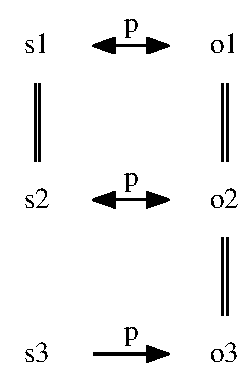
\includegraphics[width=0.4\columnwidth]{./img/fixpoint_example_cropped}
\caption{
  An illustrative example showing that defining
  $\lowerapprox$ in terms of $\higherapprox$ may not be optimal.
  The identity relation is represented with double-lined edges.
  $s_i$, $p$, and $o_i$ are subject, predicate, and object terms respectively.
  The directed edges represent triples.
}
\end{figure}

The indiscernibility criteria for this example are shown
  in equation \ref{eq:20}.

\begin{align}
\label{eq:20}
  \indp_{\approx}(\set{s_1,s_2,s_3})
&=\\
  \indp_{\approx}(\set{o_1,o_2})
&=
  \setdef{p^n}{\natnum{n}}\nonumber
\end{align}

\noindent Based on these indiscernibility criteria
  the naive lower approximation
  (definition \ref{def:identity_lower_approximation}) is empty.
But notice that there is a slight asymmetry in the way we have
  calculated this result.
We have defined $\lowerapprox$ in terms of $\indp_{\approx}$,
  i.e. in terms of $\approx$.
It seems more correct, however, to base the indiscernibility criteria
  for calculating the lower approximation on $\lowerapprox$ itself
  (and similarly for the higher approximation).
The resulting definition \ref{def:identity_lower_approximation_fixpoint}
  is recursive.
It affects the closure operations over the predicate and object terms
  in \mbox{definition \ref{def:indiscernibility_predicates}}.

\begin{definition}
\label{def:identity_lower_approximation_fixpoint}
\begin{align}
  x \in \lowerapprox
\, \iff \,
    \setdef{y}{x \equiv_{\indp_{\lowerapprox}} y}
  \; \subseteq \;
    \approx\nonumber
\end{align}
\end{definition}

\noindent There are now two correct solutions or fixpoints
  for the present example:

The first solution is the same as for the naive definition;
  $\lowerapprox_1 = \emptyset$,
  where $\indp_{\lowerapprox_1}(X) = \emptyset$
  for $X$ such that $\card{X} > 1$.

The second solution could not be derived in the naive case:
  $\lowerapprox_2 = \set{\pair{s_1}{s_2},\pair{o_1}{o_2}}$,
  with $\indp_{\lowerapprox_2}(\set{s_1,s_2,o_1,o_2}) = \setdef{p^n}{\natnum{n}}$
  and $\indp_{\lowerapprox_1}(X) = \emptyset$
  for all other $X$ such that $\card{X} > 1$.
This is the greatest fixpoint for this example.

Both solutions are correct,
  since both conform to the same strictures imposed by the here presented
  framework.
However, the second solution is better, since a greater fixpoint is
  to be prefered over a smaller fixpoint.
This is in line with our intuitions,
  since this enlarges the number of consistently applied identity pairs,
  as can be glanced from the quality criterion in
  \mbox{definition \ref{def:quality}}.
Reasoning along the same lines,
  a least fixpoint\footnote{
      We have no reason to believe that it should be unique.
    }
  is the best solution for the redefined higher approximation.


